%
% File          : Amjad_Ammar.tex
% Description   : A one-page introduction about me.
% Authors       : Ammar Amjad
%
% Last Modified : Sun Aug 28 12:00:00 EST 2022
%
% BDOC PARAM offset=0in,0in

% Page style
\documentclass[11pt, pdftex]{article}
\usepackage{epsf}
\usepackage{epsfig}
\usepackage{times}
\usepackage{ifthen}
\usepackage{comment}
\usepackage[margin=1in]{geometry}
\usepackage{graphicx}

\usepackage{fancyhdr}
\setlength{\parindent}{1em}

\title{ Project Report – Bitcoin Miner }
\author{ Ammar Amjad 5992-1730, Mohammad Anas 5981-5998 }
\date{ September 19, 2022 }



\begin{document}
	\pagestyle{fancy}
	\fancyhead{}
	\fancyhead[L]{Project: Bitcoin Miner}
	\fancyhead[R]{Course: DOSP COP5615}
	\fancyfoot{}
	\fancyfoot[L]{Page: \thepage}
	\fancyfoot[R]{By: Ammar Amjad, Mohammad Anas}
	\maketitle 
	
	
	\textbf{Task:} \\ 
	To make a Bitcoin miner able to mine 0’s based on the input that user enters, Outputting the required stats and messages. \\ 
	
	\textbf{Components:} \\
	1-	Server: That supervises all the worker nodes. \\
	2-	Local workers: Workers that fire up after the server is instantiated. \\
	3-	Remote workers: Added to server’s nodes as they become available. Remote workers communicate their availability to the server. \\
	
	\textbf{Instructions:} \\
	1-	Start server terminal with \texttt{erl -sname server}. \\
	2-	Complie \texttt{c(project).} \\
	3-	Run \texttt{project:server(n).} where n is the number of bitcoin zeros we want. Not only the server but the maximum number of workers the server can have will also be spawned to start mining on the server. \\
	4-	In another terminal, Start worker terminal with \texttt{erl -sname w1}. \\
	5-	Run \texttt{project:starthasher(server@IP).} where server is name of server, IP is the IP address of server. \\
	6-	Run multiple instances or same or different machines with above command at step 5. \\
	7-	Hash and the string used to find the hash, will be displayed by server when any of the workers/hashers finds the desired hash. \\
	8-	For distributed communication, we can run this on multiple machines on different PC’s, the commands are on page 3. We will additionally need to setup the connection for remote workers and an example is shown on page 4. \\
	
	\textbf{Input:} \\
	n - desired number of zeros - input from terminal\\ \\
	\textbf{Output:} \\
	1-	String used to find hash \\
	2-	The hash \\
	
	\textbf{Read Me File Statistics:} \\
	The following are the contents of the required stats of Read Me file.\\
	
	\textbf{Worker unit size:} \\
	max subset a single worker was given by server - only \textbf{1 string per hasher/node} was passed that connected to server.  \\
	The result of the string appended to the gator ID is again passed to the hashing function. This allows us to minimize needless communication between worker and server.  \\
	
	
	\textbf{Result of running program for input 4:} \\
	We ran the code for input 4 and received the following output. \\ \\
	Original Msg: aamjad;adba78f1755c3c420771d408edfa4d49dc2db83a98557a040bbbd7963 \\
	Hash: 00003ca5af47bbf62485a1232d94fcbb620240393d65ba7590dba7507f5181b3 \\
	
	\textbf{Cores:} \\
	The number of cores for finding 7 zeros was \textbf{15 on laptop locally} as shown in below figure. \\ \\
	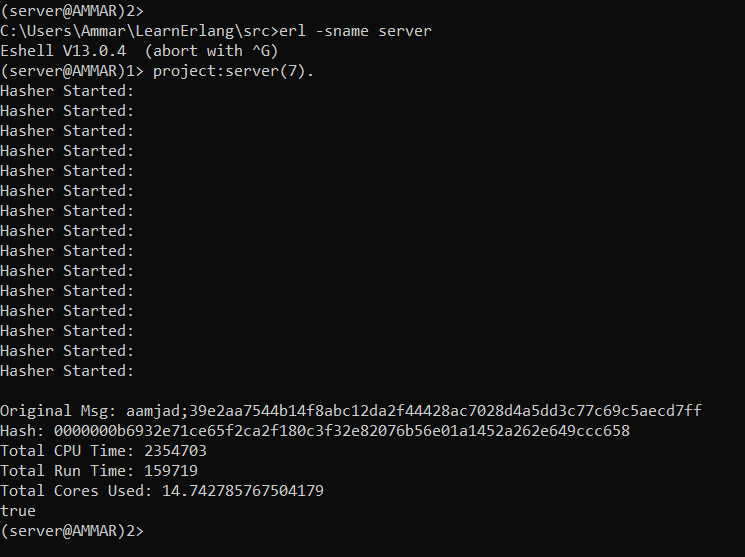
\includegraphics{Picture1.png} \\
	
	
	Another example with remote + local cores running is presented at end of this file. \\
	
	\textbf{Coins with most zeros we managed to find:}  \\
	We managed to find upto \textbf{7 zero} string, the output is shown below. \\ \\
	Original Msg: aamjad;a76f78af03eb05b819aa90f1de18cf9dcffb4d8cf06981262a008cd04 \\
	Hash: 00000006505632a55167113210e6968d6df5084459f1fcacd331a5237b00d3b2 \\ \\
	
	\textbf{Largest number of worker machines able to run code:}  \\There is no limit to connections, but the most we connected were 8 workers from remote terminals on a different pc + 15 local workers on server pc = \textbf{23 total worker nodes} working for server. \\
	
	\textbf{Commands to connect from remote PC:} \\
	Run these commands based on either windows or linux machines, Terminal must be run under administrator modes on both machines: \\
	
	\begin{verbatim}
		On both machine start terminal in administrator mode.
	
	For Linux:	
	
	Step 1:	
	Linux machine 1:
	erl -name freebsd_node1@10.20.23.44 -setcookie 'mycookie'
	Linux machine 2:
	erl -name freebsd_node2@10.20.23.37 -setcookie 'mycookie'
	Step 2:
	Linux machine 1:
	net_kernel:connect_node('freebsd_node2@10.20.23.37')
	Linux machine 2:
	net_kernel:connect_node('freebsd_node1@10.20.23.44')
	
	------------------
	For Windows:
	
	Step 1:
	Windows machine 1:
	werl -name windows_node1@10.20.23.44 -setcookie 'mycookie'
	Windows machine 2:
	werl -name windows_node2@10.20.23.37 -setcookie 'mycookie'
	Step 2:
	Windows machine 1:
	net_adm:ping('windows_node2@10.20.23.37')
	Windows machine 2:
	net_adm:ping('windows_node1@10.20.23.44')
	
	nodes( ). 
	\end{verbatim} 
	
	Executing commands above to connect to remote server, the below is a screenshot of a successful connection with a remote PC.
	
	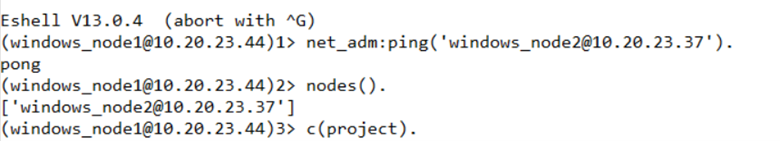
\includegraphics{Picture2.png} \\
	
	\textbf{Results for input 7 :} \\
	Here is an example where we connected remotely using the commands above and then started 15 nodes on server PC and then connecting 8 nodes from a remote PC. The output is shown below for finding 7 zero's. \\
	
	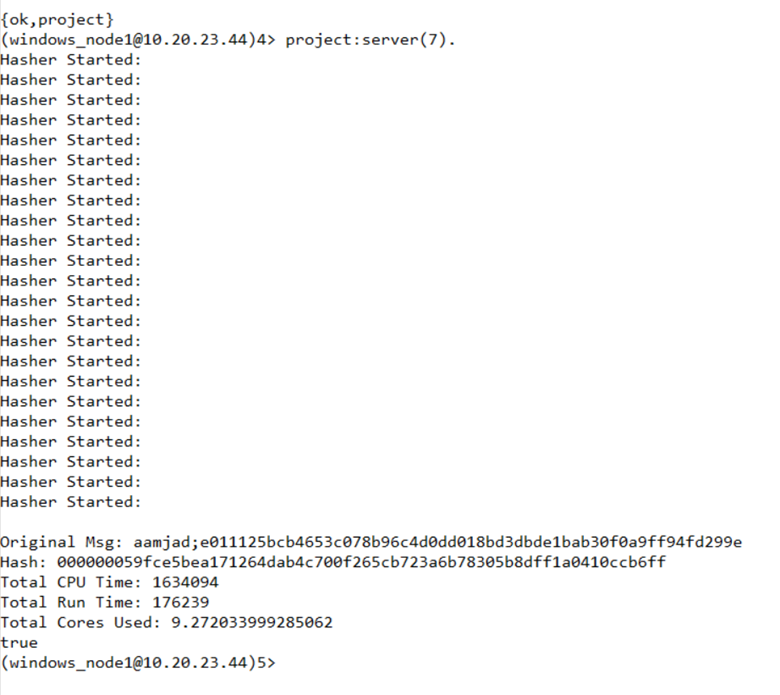
\includegraphics{Picture3.png} \\
	
	\textbf{Conclusion:} 
	
	We are able to mine 0’s based on the input that user enters, Outputting the required stats and messages.  \\
	
	\textbf{Reach out to us at for any question at:} \\
	
	
	ammar.amjad@ufl.edu
	
	5992-1730 
	
	mo.anas@ufl.edu
	
	5981-5998
	
	
	
\end{document}
